\chapter{Infraestructura}
Una vez que el proyecto y sus objetivos han sido definidos, nos centraremos en este capítulo en las tecnologías usadas para el desarrollo de la aplicación, comenzando por el marco que engloba el conjunto de subsistemas.

MEAN (acrónimo para: MongoDB, ExpressJS, AngularJS, NodeJS), es un marco o conjunto de subsistemas de software para el desarrollo de aplicaciones web, y páginas web dinámicas, que están basadas, en el popular lenguaje de programación JavaScript.

Como se observa en la imagen \ref{img:EsquemaMean}, el Frontend desarrollado con Angular, es el encargado de hacer llamadas al API REST (Post, Put, Get y Delete) desarrollado en NodeJS que utiliza el entorno Express. El API podrá hacer un CRUD (Create-Read-Update-Delete) a la base de datos MongoDB y cuando el API tenga los datos que se le han pedido en la llamada los devolverá a Angular en formato JSON y este los mostrará en pantalla, ya que Angular mantiene el modelo de datos actualizado sin necesidad de recargar la página.

\begin{figure}[!h]
    \centering
    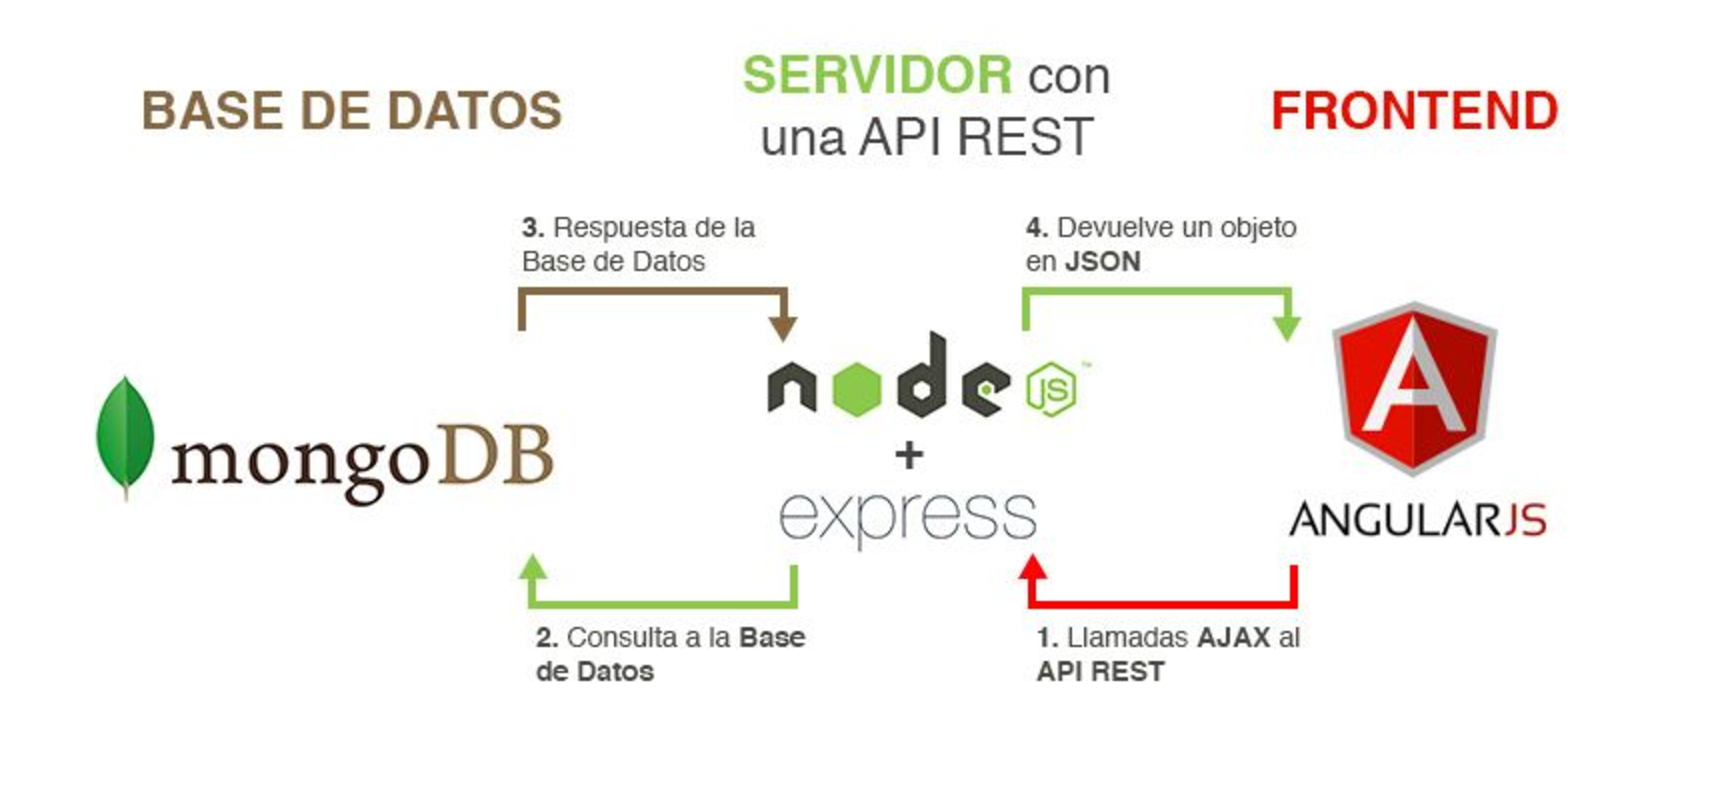
\includegraphics[width=140mm]{img/infraestructura/scheme.png}
    \caption{Esquema MEAN}
    \label{img:EsquemaMean}
\end{figure}



Las ventajas de MEAN \cite{mean} provienen de la robustez de Node, el cual proporciona su API abierta en tiempo real, que puede ser usada libremente con nuestro código \textit{frontend} en Angular.
Podemos emplearlo para transferir datos para aplicaciones como chats, actualización de estados, o cualquier otra situación que requiera mostrar datos rápidamente en tiempo real.
\section{Angular }

\begin{figure}[!h]
    \centering
    
\includegraphics[width=80mm]{img/infraestructura/a22.jpg}
    \caption{Icono de Angular}
\end{figure}


Angular \cite{angular} es un tecnología JS para la parte cliente de una aplicación web, que respeta el paradigma MVC y permite crear \textit{Single-Page Applications} (Aplicaciones web que no necesitan recargar la página), de manera más o menos sencilla. Es un proyecto mantenido por Google y que actualmente está en auge.

Angular es un entorno completo para construir aplicaciones en cliente con HTML y Typescript, es decir, con el objetivo de que el peso de la lógica y el renderizado lo lleve el propio navegador, en lugar del servidor.

Para crear apps en Angular necesitamos:

\begin{enumerate}
\item {Plantillas HTML \textit{(templates)}}
\item {Componentes para gestionar esas plantillas}
\item {Servicios para gestionar la lógica de la aplicación}
\item {El componente raíz de la aplicación al sistema de arranque de Angular \textit{(bootstrap)}.}
\end{enumerate}

En la figura \ref{img:DiagramaAngular} se puede observar como se relacionan estos elementos en el diagrama de arquitectura típico, sacado de la web de Angular:
Podemos identificar los 8 bloques principales de una aplicación web con Angular:
\begin{figure}[!h]
    \centering
    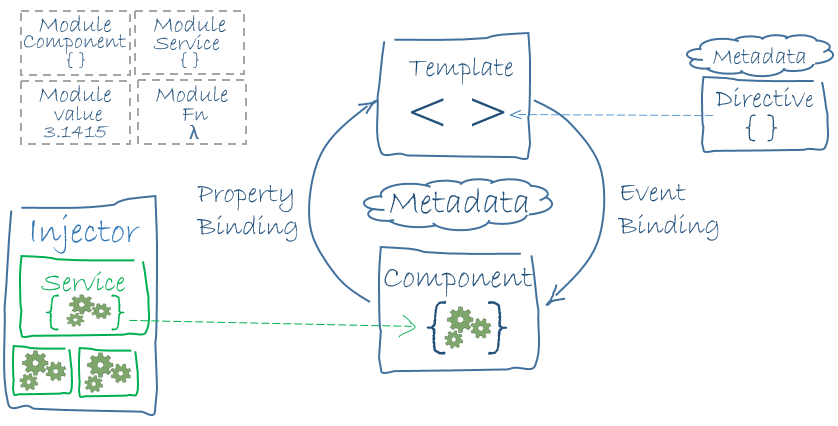
\includegraphics[width=90mm]{img/infraestructura/angular2Architecture.png}
    \caption{Diagrama de Angular}
    \label{img:DiagramaAngular}
\end{figure}



En este TFG hemos utilizado la versión 6 de Angular para programar el lado cliente de la aplicación web de clases particulares.

\subsection{Módulo}
Las aplicaciones de Angular en su versión más actualizada son modulares. Un módulo es típicamente un conjunto de código dedicado a cumplir un único objetivo. El módulo exporta algo representativo de ese código, típicamente una única cosa como una clase. Los módulos se pueden exportar e importar:

\begin{lstlisting}
//app/app.component.js
    export class AppComponent {
        //aqui va la definicion del componente
    }

//app/main.js
    import { AppComponent } from './app.component';
\end{lstlisting}

Hay módulos que son librerías de conjuntos de módulos. Las librerías principales de Angular son:


\begin{itemize}
\item \textbf{@angular/core}
\item \textbf{@angular/common}
\item \textbf{@angular/router}
\item \textbf{@angular/http}
\end{itemize}


\subsection{Componente} Un componente controla una zona de espacio de la pantalla que podríamos denominar vista. El componente define propiedades y métodos que están disponibles en su plantilla, pero eso no da licencia para meter ahí todo lo que te parezca. Haciendo un símil con AngularJS (Angular en su primera versión), un componente vendría a ser un controlador que siempre va ligado a una vista.
\subsection{Plantilla} La plantilla \textit{(template)}, permite definir la vista de un Componente de Angular en código HTML, decorado con otros componentes y algunas directivas (expresiones de Angular que enriquecen el comportamiento de la plantilla).
\begin{lstlisting}[caption=Plantilla en Angular, label=PlantillaAngular]
<h2>Todo List</h2>
<p><i>List of Tasks</i></p>
<div *ngFor="let todo of todos" (click)="selectTodo(todo)">
  {{todo.subject}}
</div>
<todo-detail *ngIf="selectedTodo" [todo]="selectedTodo"></todo-detail>
\end{lstlisting}
Como vemos en la tabla \ref{PlantillaAngular}, además de elementos HTML normales como $<$h2$>$ y $<$div$>$, hay otros elementos desconocidos \textit{(*ngForg, todo.subject, (click), [todo], todo-detail)}  que explicaremos en a sección de databinding

\subsection{Metadatos} La forma de añadir metadatos a nuestra clase en TypeScript es mediante el patrón decorador justo antes de la declaración de la clase, tal y como se muestra en la tabla \ref{MetadatoAngular}
\begin{lstlisting}[caption={Metadatos en Angular }, label=MetadatoAngular]
   import { Component } from '@angular/core';

    @Component({
      selector:    'todo-list',
      templateUrl: 'todo-list.component.html',
      styleUrls: ['todo-list.component.css'],
      moduleId:    module.id,
      directives:  [TodoDetailComponent],
      providers:   [TodoService]
    })
    export class TodoListComponent { ... }
\end{lstlisting}


\subsection{Data Binding}
Uno de los principales valores de Angular es que abstrae la lógica \textit{pull/push} asociada a insertar y actualizar valores en el HTML y permite convertir las respuestas de usuario (inputs, clicks, etc) en acciones concretas. Escribir toda esa lógica a mano (lo que típicamente se hacía con JQuery) es tedioso y propenso a errores, y Angular lo resuelve gracias al Data Binding.
Tal y como vemos en la tabla \ref{PlantillaAngular2}, podemos diferenciar los distintos tipos de Data Binding que tiene Angular.
\begin{lstlisting}[caption=Data Binding en Angular, label=PlantillaAngular2]
<h2>Todo List</h2>
<p><i>List of Tasks</i></p>
<div *ngFor="let todo of todos" (click)="selectTodo(todo)">
  {{todo.subject}}
</div>
<todo-detail *ngIf="selectedTodo" [todo]="selectedTodo"></todo-detail>
\end{lstlisting}
\begin{itemize}
\item \textbf{Interpolación} Hacia el DOM.
{{todo.subject}}
\item \textbf{Property binding} Hacia el DOM.
[todo]="selectedTodo"
\item \textbf{Event binding} Desde el DOM. (click)="selectTodo(todo)"

\item \textbf{Two-way binding} (Desde/Hacia el DOM) input [(ngModel)]="todo.subject"
\end{itemize}

Angular procesa los \textit{data binding} una vez por cada ciclo de eventos JavaScript, desde la raíz de la aplicación siguiendo el arbol de componentes en orden de profundidad.

La figura \ref{img:DatabindingAngular} ilustra la importancia del data-binding para la comunicación entre componentes, así como componente-plantilla.

\begin{figure}[!h]
    \centering
    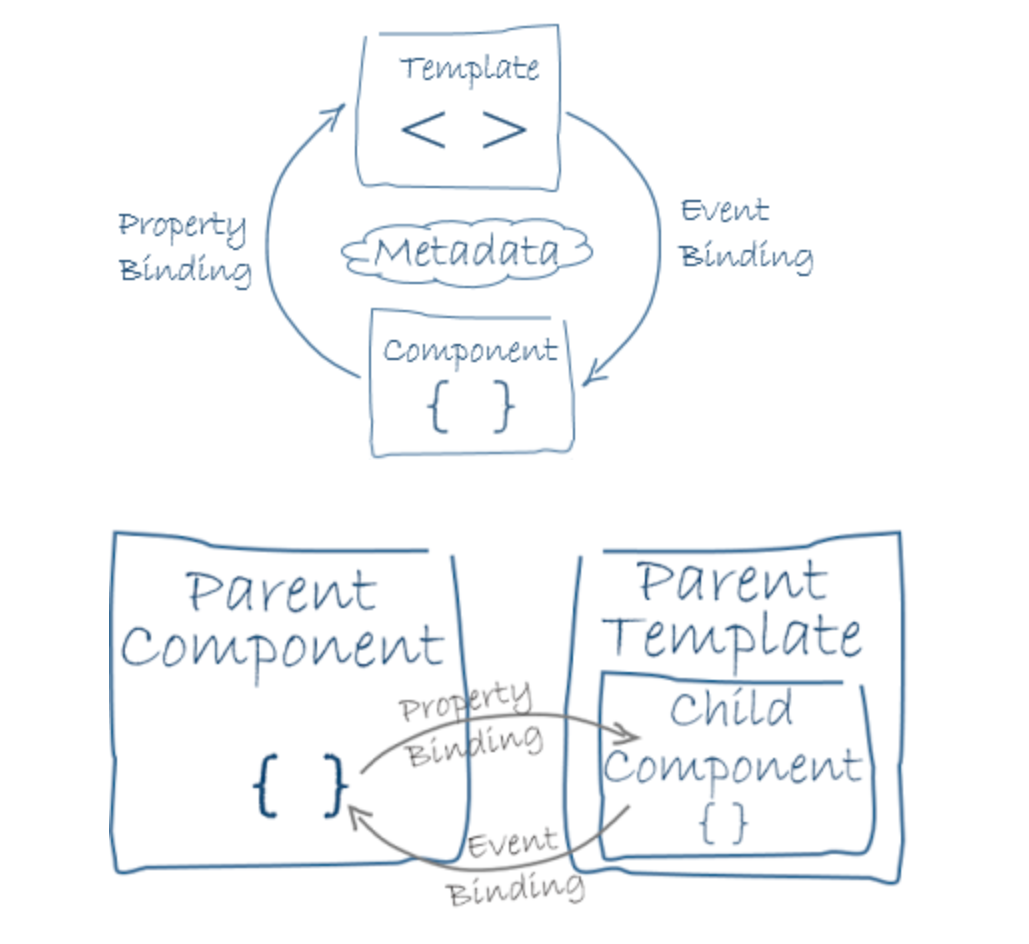
\includegraphics[width=60mm]{img/infraestructura/databinding.png}
    \caption{Data-Binding Diagrama}
    \label{img:DatabindingAngular}
\end{figure}


\subsection{Directiva}

Los plantillas de Angular son dinámicas: Cuando Angular los renderiza, transforma el DOM en base a las instrucciones que encuentra en las directivas

Un Componente es un caso concreto de directiva que siempre va asociado a una plantilla y al que por ser un elemento tan importante en Angular se le ha dado un decorador propio.

Tenemos dos tipos de directivas:
\begin{itemize}
\item \textbf{Las directivas estructurales} comienzan por asterisco y sirven para alterar el DOM.
\begin{lstlisting}[language=javascript]
   <div *ngFor="let todo of todos"></div>
    <todo-detail *ngIf="selectedTodo"></todo-detail>
\end{lstlisting}
\item \textbf{Las directivas Atributo} alteran la apariencia o comportamiento de un elemento del DOM

\begin{lstlisting}[language=javascript]
   <input [(ngModel)]="todo.subject" >
\end{lstlisting}

\end{itemize}
\subsection{Servicio }

Los servicios son imprescindibles en Angular, se definen a través de simples clases. Todo valor, función o característica que nuestra aplicación necesita, se encapsula dentro de un servicio.

Los Componentes son grandes consumidores de servicios. No recuperan datos del servidor, ni validan inputs de usuario, ni logean nada directamente en consola. Delegan todo este tipo de tareas a los Servicios.

\subsection{Inyección de Dependencias}  Una dependencia en tu código se produce cuando un objeto depende de otro. Hay diferentes grados de dependencia, pero tenerlas en exceso hace que probar tu código sea complicado o que algunos procesos se ejecuten más tiempo de la cuenta.
La inyección de dependencias es un método por el cual damos a un objeto las dependencias que requiere para su funcionamiento.


Angular permite extender el vocabulario del HTML con directivas y atributos para crear componentes dinámicos. En las páginas web dinámicas sin Angular hay ciertas complicaciones frecuentes, como el data binding, validación de formularios, manejador de eventos con DOM (Document Object Model) y otras muchas. Angular presenta una solución “todo-en-uno” a esos problemas.
La curva de aprendizaje para Angular es muy pequeña, lo que explica que mucha gente se esté pasando a este marco. La sintaxis es simple y sus principios básicos como el data binding (vinculación de elementos de nuestro documento HTML con nuestro modelo de datos) y la inyección de dependencias son sencillas de entender.

\section{Node}

\begin{figure}[!h]
    \centering
    
\includegraphics[width=80mm]{img/infraestructura/node.png}
    \caption{Icono de Node}
\end{figure}
Node\cite{nodejs} es un entorno de programación en JavaScript para el Backend basado en el motor V8 del navegador Google Chrome y orientado a eventos, no bloqueante, lo que lo hace muy rápido a la hora de crear servidores web y emplear tiempo real. Fue creado en 2009 y aunque aún es joven, las últimas versiones lo hacen más robusto. Además posé una gran comunidad de desarrolladores.

Uno de los beneficios de Node es su gestor de paquetes, npm (node package manager), el cual nos permite gestionar todas las dependencias y módulos de una aplicación. Al igual que Ruby tiene RubyGems y PHP tiene Composer, Node tiene npm.
Viene ya incluido con Node y permite bajar una serie de paquetes para satisfacer la necesidades del servicio programado.
Este sistema de paquetes es lo que hace a Node tan potente. La capacidad de tener una serie de códigos que puedes reutilizar en todos tus proyectos hace que el desarrollo sea más sencillo, ya que puedes combinar facilmente varios paquetes para crear aplicaciones complejas.

\begin{lstlisting}
    > npm install && npm start
\end{lstlisting}

Con esta instrucción en linea de comandos, nos descargamos todas las dependencias, además de arrancar nuestra aplicación.
En este TFG se ha utilizado Node para programar el servidor web de la aplicación de gestión de clases particulares.


\section{MongoDB}
\begin{figure}[!h]
    \centering
    
\includegraphics[width=40mm]{img/infraestructura/mongo2.png}
    \caption{Icono de MongoDB}
\end{figure}

MongoDB\cite{mongodb} es la base de datos que ha elegido para la aplicación de gestión de clases particulares, debido a sus grandes ventajas cuando se manejan ingentes cantidades de información. MongoDB nace en octubre de 2009 y a día de hoy innumerables empresas ya disponen de esta base de datos en sus aplicaciones como por ejemplo:
\begin{itemize}
\item \textbf{Bosh:} Utiliza MongoDB ya que está poniendo a prueba una aplicación que es capaz de capturar datos de vehículos, como el sistema de frenado, la dirección asistida, los limpiaparabrisas ... Con todos estos datos se pueden hacer diagnósticos de necesidad de mantenimiento preventivo.


\item \textbf{Forbes:} Construyó todo un sistema de gestión de contenidos en MongoDB. Además utiliza MongoDB para analítica en tiempo real. Cuando algún artículo se hace viral, Forbes detecta la forma en que se está compartiendo entre los usuarios y de este modo sabe qué tipo de contenido le debe ofrecer a sus lectores.
\end{itemize}

\subsection{Características}
MongoDB es una base de datos no relacional (NoSQL) de código abierto que guarda los datos en documentos tipo JSON (JavaScript Object Notation) pero en forma binaria (BSON) para hacer la integración de una manera más rápida. Se pueden ejecutar operaciones en JavaScript en su consola en lugar de consultas SQL. Además tiene una gran integración con Node.js con los drivers propios y con Mongoose. Debido a su flexibilidad es muy escalable y ayuda al desarrollo ágil de proyectos web.

MongoDB está orientado a servicios que necesiten una persistencia basada en documentos, al contrario que otros sistemas de base de datos noSQL como Cassandra, el cual esta orientado a logs, o como Redis que necesita una persistencia basada en colas de mensajes.

Actualmente estamos en la era de lo que Martin Fowler llama “Polyglotpersistence”. Hay que decidir el tipo de persistencia a utilizar para después usar el tipo de persistencia que más se amolde a nuestras necesidades.

Las características que hacen tan importante a esta base de datos son las siguientes:



\begin{itemize}

    \item Está orientada a documentos. En un único documento es capaz de almacenar toda la información necesaria que define un producto, un cliente, etc, aceptando todo tipo de datos sin tener que seguir un esquema predefinido.

    \item Da respuesta a la necesidad de almacenamiento de todo tipo de datos: estructurados, semi estructurados y no estructurados.

    \item Tiene un gran rendimiento en cuanto a escalabilidad y procesado de la información. Puede procesar la gran cantidad de información que se genera hoy en día.

    \item Permite a las empresas ser más ágiles y crecer más rápidamente, creando así nuevos tipos de aplicaciones.


\end{itemize}


\subsection{Documento en MongoDB}
MongoDB está escrito en C++, su versión de 32 bits sólo puede alcanzar 2GB, por este motivo la versión de 32 bits no es recomendable usarla en producción.
\begin{lstlisting}
{
    name: "mario",
    age: 25,
    preferences: [
        "programming",
        "nosql",
        "javascript"
    ]
}

\end{lstlisting}


Esto es un documento en Mongo, los cuales se almacenan en colecciones y éstas a su vez en bases de datos. Estas colecciones poseen un esquema flexible y totalmente dinámico lo que hace que la velocidad de cómputo sea muy alta. Las bases de datos no se crean manualmente, primero se define la base de datos a usar y luego se inserta un documento en alguna colección.

\begin{lstlisting}
    > show dbs
    > use pruebanosql
    > show colections
    > db.users.insert({"name":"mario", "age":24})
\end{lstlisting}

\subsection{Inconvenientes de MongoDB}
Un problema que tiene Mongo es que no soporta transacciones de múltiples documentos. Sin embargo puede proporcionar operaciones atómicas en un solo documento. A menudo estas operaciones atómicas de nivel de documento son suficientes para resolver los problemas que requerían transacciones en una base de datos relacional. Por ejemplo, en Mongo se pueden incrustar datos relacionados en matrices anidadas o documentos anidados dentro de un solo documento y actualizar todo el documento en una sola operación atómica. Por este motivo los servicios que requieren de transacciones, como los bancos o entidades económicas, no utilizan Mongo debido a que no es capaz de hacer una sola operación atómica en dos documentos.

Otro posible problema es la excesiva cantidad de memoria RAM que puede consumir MongoDB, aunque es posible ejecutar MongoDB en una maquina con una pequeña cantidad de memoria RAM libre. MongoDB usa automáticamente toda la memoria libre del equipo como su cache, es por esto por lo que los monitores de recursos muestran que MongoDB utiliza una gran cantidad de memoria, pero su uso es dinámico. Es decir que si otro proceso de repente necesita mayor espacio de memoria RAM, MongoDB liberará parte de su memoria asignada para el otro proceso.

\subsection{Fragmentación \textit{(Sharding)}}
\begin{figure}[!h]
    \centering
    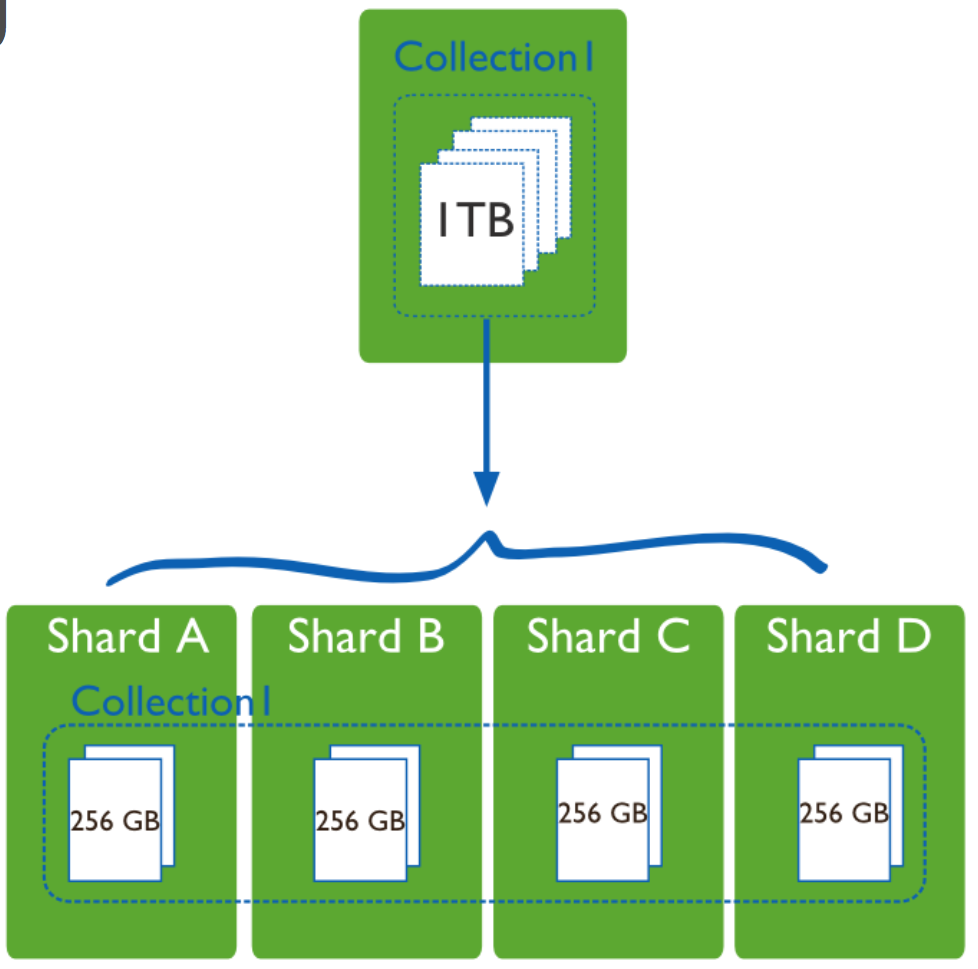
\includegraphics[width=90mm]{img/infraestructura/shard.png}
    \caption{Sharding}
\end{figure}
¿Que es la fragmentación?
Cuando un proyecto empieza a tener un número de peticiones de acceso elevado , se empieza a notar que su base de datos va más lento de lo normal. Para este problema se tiene dos soluciones, una actualizar toda la infraestructura para soportar la demanda o empezar a utilizar la fragmentación.

La fragmentación, es el modo en el se hace la base de datos escalable. En lugar de tener una colección en una base de datos, se tendría en varias bases de datos distribuidas, de modo que a la hora de consultar los datos de dicha colección, se recupera como si de una única base de datos se tratase. Esto de encontrar la base de datos lo hace MongoDB de forma transparente. Cuando se hacen consultas, se tiene un enrutador llamado "MongoS", el cual mantendrá un pequeño conjunto de conexiones a los distintos fragmentos.

Los fragmentos estarán formados por \textit{réplica set}, de modo que si creamos tres fragmentos, cada uno de los cuales tiene una \textit{réplica set} con tres servidores, estaríamos hablando de un total de nueve servidores. Para saber en qué fragmento debe consultar para recuperar datos de una colección ordenada, se utilizan rangos y \textit{shard key}, de modo que se trocea la colección en rangos y se les asigna un identificador a cada rango. De este modo cuando se consulte la colección debemos proporcionar el \textit{shardKey}.

\section{Express}

\begin{figure}[!h]
    \centering
    
\includegraphics[width=90mm]{img/infraestructura/express2.png}
    \caption{Icono de Express}
\end{figure}

\subsection{Introducción}
Express \cite{express} es un entorno de aplicaciones web para Node.js, que permite crear servidores web y recibir peticiones HTTP de una manera sencilla, lo que permite también crear APIs REST de forma rápida.

En la web de ExpressJS, se describe como \textit{un entorno de desarrollo de aplicaciones web minimalista y flexible para Node.js}. Sin duda el éxito de Express radica en lo sencillo que es usarlo, y además abarca un sin número de aspectos que muchos desconocen pero son necesarios.

La referencia de la API se divide en 5 grandes módulos:

\begin{itemize}

\item \textbf{express():} La función \textit{express()} es una función de nivel superior exportada por el módulo express.
\begin{lstlisting}
    express.json()
    express.static()
    express.Router()
    express.urlencoded()
\end{lstlisting}
\item \textbf{Application:} El objeto \textit{app} se crea llamando a la función express () de nivel superior exportada por el módulo Express
\begin{lstlisting}
Properties -->|app.locals||app.mountpath|
Events -->| mount|
Methods -->|app.all()|app.delete()|app.disable()|app.listen()|
\end{lstlisting}
\item \textbf{Request:} El objeto \textit{req} representa la solicitud HTTP y tiene propiedades para la cadena de consulta de solicitud, parámetros, cuerpo, encabezados HTTP, etc.
\begin{lstlisting}
Properties -->|req.body|req.cookies|
Methods -->|req.accepts()|req.acceptsCharsets()|
\end{lstlisting}
\item \textbf{Response:} El objeto \textit{res} representa la respuesta HTTP que envía una aplicación Express cuando recibe una solicitud HTTP.
\begin{lstlisting}
Properties -->|res.app|res.headersSent|res.locals|
Methods -->|res.cookie()|res.clearCookie()|
\end{lstlisting}
\item \textbf{Router:} El objeto \textit{Router} es una instancia aislada de middleware y rutas. Puede considerarlo como una "miniaplicación", que solo puede realizar funciones de enrutamiento y middleware. Cada aplicación Express tiene un router de aplicaciones integrado.
\begin{lstlisting}
Methods -->|router.all()|router.METHOD()|router.param()|
\end{lstlisting}
\end{itemize}


\subsection{Estructura de una API}

En una aplicación escrita con express existe una estructura interna bien definida y es como sigue:


\begin{itemize}

    \item \textbf{Módulos o archivos externos} Importamos todos los módulos o archivos externos que nuestra app vaya a necesitar. El bloque, o mejor dicho la línea, que viene a continuación es la más importante de todas, ya que se encarga de instanciar Express y asignarlo a la variable app, la cual se utilizará a partir de ahora para configurar los parámetros de Express.

    \begin{lstlisting}
    var app = express();
   \end{lstlisting}

   El siguiente bloque sirve para configurar e iniciar algunos componentes de Express. Destacar la línea, \textit{app.use(express.static(...))}, en la cual se configuran los objetos estáticos (imágenes, hojas de estilo, etc.) que debe servir Express, los cuales se encuentran en la carpeta \textit{public}. Esta configuración permite también que los elementos estáticos puedan ser accedidos como si se encontrasen en el directorio raíz del proyecto, de forma que para acceder a las imágenes ubicadas en /public/images se haría con la URL http://localhost:3000/images.
    \begin{lstlisting}
    app.use(bodyParser.json());
    app.use(bodyParser.urlencoded({ extended: false }));
    app.use(cookieParser());
    app.use(express.static(path.join(__dirname, 'public')));
   \end{lstlisting}


    \item \textbf{Conectamos a la base de datos} La segunda parte de nuesta app \textit{express} es conectarnos a la base datos.

    \item \textbf{Importamos controladores y modelos de la base de datos} Una vez conectados a la base de datos importamos los controladores y los modelos de nuestra base de datos.


   \item \textbf{Rutas} Las rutas son definitivamente la parte más importante de tu aplicación, ya que son las encargadas de invocar las funciones que se encuentran en el controlador.

   Una ruta está especificada de la siguiente forma:
   \begin{lstlisting}
    app.VERBO(PATH, ACCION)
   \end{lstlisting}

   VERBO: Puede ser: GET, POST, PUT, DELETE y así para cada uno de los verbos HTTP.

   PATH: Define la dirección de acceso.

   ACCION: Que es lo que se tiene que hacer.

   \item \textbf{Listen} Por último, es importante que la aplicación esté disponible en algún puerto.
   \begin{lstlisting}
    app.listen(8000);
   \end{lstlisting}

\end{itemize}

Express esconde muchas funcionalidades internas de Node, lo que permite sumergirse en el código de la aplicación y conseguir los objetivos de forma muy rápida. Es fácil de aprender y deja cierta flexibilidad con su estructura.
Por algo es el entorno más popular de Node.
\section{Amazon web services}

\begin{figure}[!h]
    \centering
    
\includegraphics[width=40mm]{img/despliegue/aws2.png}
    \caption{AWS}
\end{figure}

Amazon Web Services es el proveedor más famoso y más completo en infraestructura como servicio (IaaS), ya que ofrece un conjunto de servicios y un modelo de precios muy completo y que se ajusta a las necesidades de cada cliente.

Dispone de varios tipos de instancias según su hardware:

\begin{enumerate}
    \item \textbf{Instancias estándar: } Pequeñas, medianas, grandes y extra-grandes
    \item \textbf{Instancias con gran cantidad de memoria}
    \item \textbf{Instancias con CPU de alto rendimiento}
    \item \textbf{Instancias en cluster: } Con redes de alta velocidad ente ellas
    \item \textbf{Instancias de GPU para clústeres}
\end{enumerate}

Además Amazon Web Services dispone de diferentes servicios entre los que destacamos:
\begin{enumerate}
    \item \textbf{Amazon Elastic Block Store: } Disco duro de las instancias persistente, donde sus datos permanecen cuando la instancia se apaga.
    \item \textbf{Varias ubicaciones: }El cliente puede elegir la ubicación para reducir la latencia a los usuarios de los servicios. Además, existen varias zonas de disponibilidad dentro de la misma ubicación para minimizar el impacto de las catástrofes.
    \item \textbf{Direcciones Elastic IP: }Por defecto las instancias tienen IPs internas en la red de Amazon, asociando una IP pública a una instancia.
    \item \textbf{Amazon Cloud Watch: }Servicio de monitorización de instancias con sistema de alarmas y gráficas de uso de recuros (memoria, CPU, red...)
    \item \textbf{Auto Scaling: } Se pueden configurar reglas para que Amazon inicie más instancias cuando la carga de las existentes supere un umbral y volver a bajar cuando la carga disminuya.
    \item \textbf{Elastic Local Balancer: } Dispositivos que reparten las peticiones web a cada una de las instancias que se han creado con el escalado automático o manual.
    \item \textbf{Imágenes de Instancias (AMI): } Amazon permite la gestión de las instancias (AMI), pudiendo crear y gestionar varias imágenes. Se puede iniciar una instancia con cualquier imagen.
\end{enumerate}
